\section{Theory and methodology}\label{sec:metho}

\subsection{Probe setup}\label{subsec:metho-mats}
The \ac{oecp} used in this project was developed by PhyVertX Technologies Inc., and is an adaptation for higher frequencies of the probe described in \parencite{Filali2008} which was tested on different substrates such as vegetation, snow and ice, and soil \parencite{Mavrovic2018,Mavrovic2020,Mavrovic2021}.
The probe is made of two conducting coaxial cylinders with a \ac{ptfe} core akin to a coaxial cable.
The inner cylinder has a \(2a =\) \SI{4}{\mm} diameter while the outer cylinder diameter is \(2b =\) \SI{13.2}{\mm} (Figure~\ref{fig:probe-scheme}A).

\begin{figure}[ht!]
    \centering
    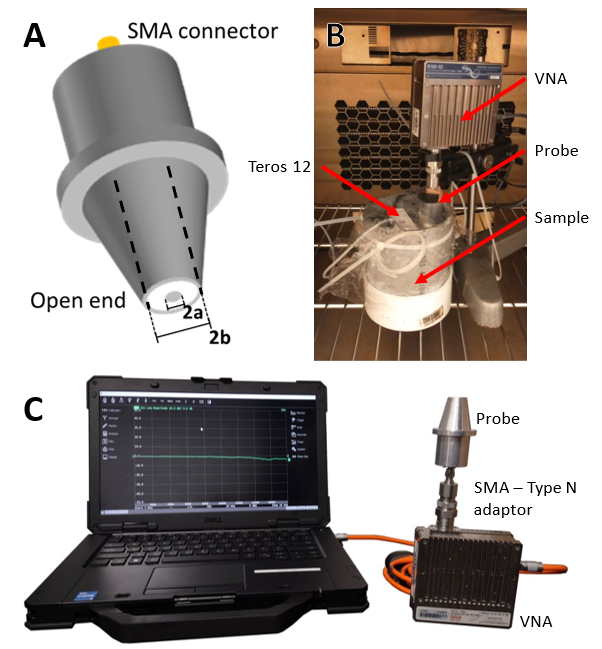
\includegraphics[width=0.9\columnwidth]{Images/method-pic.png}
    \caption[]{\textbf{A:} \ac{oecp} scheme, where the diameter of the conductive core (2a) is \qty{4}{\milli\meter} and the outer diameter of the PTFE core (2b) is \qty{13.2}{\milli\meter}; \textbf{B:} Experimental setup for the temperature cycle measures; \textbf{C:} \ac{vna} and \ac{oecp}, connected to the computer with the operating software for the \ac{vna}}\label{fig:probe-scheme}
\end{figure}

The probe's dimensions were chosen sufficiently large for the measurement of heterogeneous material such as soil while being able to cover a frequency range from \SI{0.5}{\giga\hertz} up to \SI{18}{\giga\hertz}.
To operate the \ac{oecp}, a \(1\)-port \acf{vna}, the R180 (\SIrange{0.001}{18}{\giga\hertz}, frequency resolution of \qty{50}{\hertz}) from Copper Mountain\(^\text{\textregistered}\) Technologies was used.
All the instruments, connectors and cables in the setup have an impedance of \SI{50}{\ohm} to reduce unwanted reflections.
In order to connect the \ac{oecp} (SMA connector) to the \ac{vna} (Type-N connector), a solid adaptor was used to eliminate possible noise that could occur in cables or semi-rigid adaptors.
The \ac{vna} was then connected to a computer and was operated by the RVNA software distributed by the company (Figure~\ref{fig:probe-scheme}C).
Once the setup assembled, two calibrations were performed to ensure the accuracy of the measurements: the first calibrates the cables and connectors connected to the probe using a specific calibration kit (system calibration) and the second calibrates the probe measurement plane, i.e.\ the aperture of the probe (probe calibration, see Section~\ref{subsec:metho-calib} for more details).

\subsection{Probe measurement principle}\label{metho:probe-princip}
In order to obtain the permittivity at the aperture of the probe, the \ac{vna} measures the reflection coefficient \(\rho\).
This measured reflection coefficient \(\rho\) is then linked to the real reflection coefficient \(\Gamma\) through the scattering parameters of the probe with the Equation~\ref{eq:gamma-sij} \parencite{Nyshadham1992}:
%
\begin{equation}\label{eq:gamma-sij}
    \Gamma = \frac{\rho-S_{11}}{S_{22}\rho+S_{12}S_{21}-S_{11}S_{22}}
\end{equation}
%
Where the \(S_{i,j} \left(i,j \in \left\{1,2\right\}\right)\) are the probe scattering parameters.
The probe calibration, detailed in Section~\ref{subsec:metho-calib}, is made to find those \(S_{i,j}\) using liquids of known permittivity.
\(\Gamma\) is also related to the admittance of both the probe (\(Y_0\)) and the material under test (\(Y(\varepsilon)\)) with Equation~\ref{eq:gamma-admit} \parencite{Nyshadham1992}:
%
\begin{equation}\label{eq:gamma-admit}
    \Gamma = \frac{Y(\varepsilon) - Y_0}{Y(\varepsilon) + Y_0}
\end{equation}
%
Finally, the permittivity of the medium (\(\varepsilon_r\)) can be deduced from its admittance (\(Y(K)\)) by solving Equation~\ref{eq:probe-permittivity} \parencite{Galejs1969a}:
%
\begin{equation}\label{eq:probe-permittivity}
    Y(K) = \frac{\varepsilon_r Z_\nu}{\ln(\sidefrac{a}{b})} 
    \int_{0}^{\infty}
    \frac{{\left[J_0(\beta p)-J_0(\alpha p)\right]}^2} % checktex 3
         {p\sqrt{\varepsilon_r - p^2}}dp
\end{equation}
%
Where \(K=\sidefrac{2\pi f}{c}\) is the wave number in vacuum, \(Z_\nu=\sqrt{\sidefrac{\mu_{0}}{\varepsilon_{0}}}\approx \qty{376.7303}{\ohm}\) is the vacuum impedance, \(\alpha = Ka\), \(\beta = Kb\) are geometric parameters, \(J_{0}\) is the zero\textsuperscript{th} order Bessel function of the first kind and \(p\) is the integration variable.  % related to the sine and cosine directors: \(p^2=u^2+v^2\).

\subsection{Calibration}\label{subsec:metho-calib}
Both calibration principles are based on the \ac{sol} one-port method, where measurements of known standards are compared to their theoretical values for all three calibration standards (open, short-circuit and load).
The measurements are then processed in order to find the \(S_{i,j}\) (Equation~\ref{eq:gamma-sij}) parameters of the calibration plane.
To obtain accurate measurements, two calibrations are necessary, the first, the system calibration, is made at the probe connection plane to calibrate the \ac{vna} and the connectors and cables connected to the probe.
For this first calibration, a S2611 calibration kit from Copper Mountain\(^\text{\textregistered}\) Technologies is used.
The kit connectors have a \SI{50}{\ohm} impedance and includes all the necessary standards.
Once the system is calibrated, the probe is connected at the end of the line and is also calibrated.

The probe calibration was made specifically for the probe using the \ac{sol} method at the measurement plane (the aperture).
The open standard corresponds to a measure in the air, the short-circuit standard was made by covering the probe with a conducting metal such as copper and the load standard was a saline (NaCl) water solution (\qty{35}{ppm}).

Using these three standards, Equation~\ref{eq:gamma-sij} can be written for each \(\rho_{1,2,3}\) and \(\Gamma_{1,2,3}\), where \(\Gamma_{1,2,3}\) is deduced from \(Y_{1,2,3}\) using Equation~\ref{eq:gamma-admit}.
Solving these three equations leads to a system of three equations for three unknown variables (Equation~\ref{eq:sij-system}):

{\footnotesize
\begin{equation*}
    S_{11} = \frac{\Gamma_1\Gamma_2\rho_3(\rho_1-\rho_2) + 
                   \Gamma_1\Gamma_3\rho_2(\rho_3-\rho_1) + 
                   \Gamma_2\Gamma_3\rho_1(\rho_2-\rho_3)}
                  {\Gamma_1\Gamma_2(\rho_1-\rho_2) + 
                   \Gamma_1\Gamma_3(\rho_3-\rho_1) +
                   \Gamma_2\Gamma_3(\rho_2-\rho_3)}
\end{equation*}
%
\begin{equation}\label{eq:sij-system}
    S_{22} = \frac{\Gamma_1(\rho_2-S_{11}) + \Gamma_2(S_{11}-\rho_1)}       
                  {\Gamma_1\Gamma_2(\rho_2-\rho_1)}
\end{equation}
%
\begin{equation*}
    S_{12}S_{21} = \frac{(\rho_1-S_{11})(1-S_{22}\Gamma_1)}{\Gamma_1}
\end{equation*}}%

After the probe calibration, two test liquids were used to assess the probe calibration quality.
The first test liquid was a saline solution at \qty{20}{ppm} and the second one was methyl hydrate.
Both computed permittivity were compared to the theoretical permittivity provided by \textcite{Nyshadham1992}.

\subsection{Data processing}\label{subsec:metho-smooth}
For every measurement presented in this work, the raw data frequency ranged from \SIrange{0.5}{18}{\giga\hertz} with increments of \SI{4}{\mega\hertz}. 
For the probe calibration and tests liquids, the permittivity was computed using the full raw data range.
Afterwards, in order to accelerate the permittivity computation for the studied samples (wet and dry paper, wet and dry sand, and soil), the raw data was truncated so that the frequency increments were of \SI{100}{\mega\hertz} over the range of \SIrange{0.5}{18}{\giga\hertz}.
This reduced the dataset size, making the computation faster while keeping a sufficient amount of data points to represent the possible variation in the permittivity.
Once the permittivity computed, the results were smoothed using the rolling window average or the exponentially weighted moving average methods with a window size of \qty{8.33}{\percent} of the total range to improve the consistency between measurements.
% For the calibration liquids, the rolling window size was \SI{1492}{\mega\hertz} or \SI{373}{points} which corresponds to 1/12th or \SI{8.3333}{\percent} of the total frequency range (\SIrange{0.5}{18}{\giga\hertz} with steps of \SI{4}{\mega\hertz}).
% For the samples with \SI{100}{\mega\hertz} increments the same rolling window size of \SI{1492}{\mega\hertz} was used but consisted of \SI{15}{points} (1/12th of the total range).

% \subsection{Highlighted frequencies}\label{subsec:mehto-freq}
Since our probe covers a wide frequency range (from \qtyrange{0.5}{18}{\giga\hertz}), the analysis was made on specific frequencies used in \ac{swe} remote sensing.
Moreover, in the context of the new satellite mission concept for \ac{swe} monitoring (\ac{tsmm}), the targeted frequencies were also added to the list (Table~\ref{tab:freq-range}).

\begin{table}[ht!]
    \centering
    \caption{Frequency bands (\qty{\pm0.25}{\giga\hertz}) on which the average permittivity was computed with examples of relevant satellite-based sensors}\label{tab:freq-range}
    \begin{tabular}{r l c c}
        Band & Frequency & Satellite example & Ref. \\
        \midrule\midrule
        L-band & \qty{1.5}{\giga\hertz} & SMOS (\qty{1.4}{\giga\hertz}) & \parencite{Kerr2010}\\
        C-band & \qty{6.9}{\giga\hertz} & RadarSAT (\qty{5.3}{\giga\hertz}) & \parencite{Morena2004} \\
        X-band & \qty{10.65}{\giga\hertz} & TerraSAR-X (\qty{9.65}{\giga\hertz}) & \parencite{Werninghaus2010} \\
        Ku-band 1 & \qty{13.5}{\giga\hertz} & TSMM (\qty{13.5}{\giga\hertz}) & \parencite{Derksen2019,Garnaud2019} \\
        Ku-band 2 & \qty{17.2}{\giga\hertz} & TSMM (\qty{17.2}{\giga\hertz}) & \\
    \end{tabular}
\end{table}

\subsection{Probe signal penetration depth}\label{subsec:metho-paper}
In order to estimate the probe penetration depth, a test using stacked paper sheet was done \parencite{Elrayes1987}.
The procedure consisted in progressively stacking sheets of paper on top of a conductive metal plate (copper, high reflectivity).
Every few sheets of paper, a permittivity measurement of the paper stack (low relative permittivity) was made.
Once the measured permittivity remained constant for additional sheets of paper, it was assumed that the signal contribution from the conductive plate was completely lost, hence the penetration depth of the probe signal was estimated.
This test was repeated for dry and wet paper on \qtyproduct{216 x 279}{\mm} (\qtyproduct{8.5 x 11}{in}) US letter size printer paper of \qty{0.1}{\milli\metre} thickness. % chktex 29

\subsection{Soil sample characterization}\label{subsec:metho-soil}
The probe was used to characterize dry and wet commercial sand and arctic organic mesic soil from Cambridge Bay, Nunavut, Canada (\ang{69.2275}, \ang{-104,8937}).
The arctic soil sample was collected using a cylindrical PVC soil sample holder of \qty{5}{\cm} radius and \qty{10}{\cm} height driven in the soil and excavated so the soil remained undisturbed.
The wet sand and organic soil samples were exposed to a temperature ramp from \qtyrange{-20}{20}{\degreeCelsius} over 10 hours inside a Climats EX-CAL 1411-HE climatic chamber at Laboratoire de l'Intégration du Matériau au Système (IMS, Bordeaux, France).
The wet sand and wet organic soil samples were placed in the convection centre of the climatic chamber (Figure~\ref{fig:probe-scheme}B).
A plastic wrap was used to seal the soil sample cylinder to ensure a constant soil moisture throughout all the temperature cycle.
To monitor the soil moisture and soil temperature during the tests, a thermocouple connected to the test chamber was used, as well as a Teros 12 (operating frequency of \qty{70}{\mega\hertz}) soil moisture and temperature probe (METER Group, Inc. USA).
The test chamber thermocouple has an approximate length \qty{4}{\cm} and was inserted in the top layer of the soil sample.

% The dry sand was also tested inside the climatic chamber using the temperature ramp and the same experimental setup, however its permittivity did not fluctuate with temperate.
% Moreover, since the sand was tested in the climatic chamber, it was subjected to a constant flow of dried air.
% No plastic wrap was used to seal the sample holder in order to maintain the dryness.
% Hence, the dry sand permittivity results shown represent the real and imaginary permittivity over all the probe frequency range.
